\documentclass[./../main.tex]{subfiles}
\graphicspath{{img/}}
\begin{document}
    % \problempts{20}

    \section{}

    Sea \(U\) el circuito dado por el siguiente diagrama:

    \begin{figure}[htb]
        \centering
        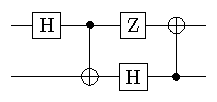
\includegraphics[scale=1.5]{cuarto-circuito.pdf} 
        \label{fig:cuarto-circuito}
    \end{figure}

    Calcule y escriba un circuito cuántico que corresponda a la operación \(U^{-1}\).

    \startsolution

    Antes de poder escribir \(U\), recordemos cómo se interpretan las compuertas aplicadas en serie (\cref{fig:compuertas-en-serie}) y paralelo (\cref{fig:compuertas-en-paralelo}).

    \begin{figure}[htb]
        \centering
        \includegraphics[scale=1.4]{compuertas-en-serie.pdf} 
        \caption{Dos compuertas \(\op{Y}\) y \(\op{X}\) aplicadas en serie. El orden en el que aparecen en el cable se invierte al multiplicarse sus matrices asociadas.}
        \label{fig:compuertas-en-serie}
    \end{figure}

    \begin{figure}[htb]
        \centering
        \includegraphics[scale=1.3]{compuertas-en-paralelo.pdf} 
        \caption{Dos compuertas \(\op{Y}\) y \(\op{X}\) aplicadas en paralelo son equivalentes a la compuerta \(\op{Y} \otimes \op{X}\).}
        \label{fig:compuertas-en-paralelo}
    \end{figure}

    A partir de lo anterior, podemos escribir la operación asociada al circuito \(U\) como:

    \begin{equation*}
        U = CNOT(\tensprod{\op{Z}}{\op{H}})\cdot CNOT(\tensprod{\op{H}}{\op{I}}).
    \end{equation*}

    Para obtener \(U^{-1}\), recordemos que para operadores unitarios se \(U^{-1} = \hc{U}\), por lo tanto

    \begin{align*}
        U^{-1} &= \Bigl[\mathrm{CNOT}(\tensprod{\op{Z}}{\op{H}})\cdot \mathrm{CNOT}(\tensprod{\op{H}}{\op{I}})\Bigr]^{\dagger},\\
        &= \bigl(\mathrm{CNOT}(\tensprod{\op{H}}{\op{I}})\bigr)^{\dagger} \cdot \bigl(\mathrm{CNOT}(\tensprod{\op{Z}}{\op{H}})\bigr)^{\dagger},\\
        &= \bigl((\tensprod{\hc{H}}{\hc{I}})\mathrm{CNOT}^{\dagger}\bigr)\cdot \bigl((\tensprod{\hc{Z}}{\hc{H}})\mathrm{CNOT}^{\dagger}\bigr),\\
        \Aboxedmain{U^{-1} &= (\tensprod{\op{H}}{\op{I}})\mathrm{CNOT}\cdot (\tensprod{\op{Z}}{\op{H}})\mathrm{CNOT}.}
    \end{align*}

    La operación \(U^{-1}\) puede representarse mediante el siguiente circuito:

    \begin{figure}[htb]
        \centering
        \includegraphics[scale=1.5]{inverse-circuit.pdf}
        \label{fig:inverse-circuit}
    \end{figure}
\end{document}
